\documentclass[a4paper,11pt]{article}
\usepackage{ctex}
\usepackage{enumerate}
\usepackage{times}
\usepackage{mathptmx}
\usepackage{amsmath}
\usepackage{amssymb}
\usepackage{tikz}
\usepackage{clrscode3e}
\usepackage[top=2cm, bottom=2cm, left=2cm, right=2cm]{geometry}

\allowdisplaybreaks[4]
\renewcommand{\labelenumi}{\textbf{\emph{\alph{enumi}}.}}
\begin{document}
  \title{����~2-7~��ҵ}
  \author{��������ۿԴ \and ѧ�ţ�161240004}
  \date{}
  \maketitle

  \section{[TC] Problem 7.1-2}
  The procedure returns $r$ when all elements in the array have the same value.

  \begin{codebox}
      \Procname{$\proc{Modified-Partition}(A, p, r)$}
      \li $x \gets A[r]$
      \li $i \gets p-1$
      \li \For $j \gets p$ \To $r-1$
      \li \Do
          \If $A[j] \leq x$
      \li \Do $i \gets i+1$
      \li exchange $A[i]$ with $A[j]$
          \End
          \End
      \li exchange $A[i+1]$ with $A[r]$
      \li $j \gets i$
      \li \While $j \geq p$ and $A[j] \isequal A[i]$
      \li \Do $j \gets j-1$
          \End
      \li \Return $\lfloor(i+j)/2\rfloor$
    \end{codebox}

  \section{[TC] Problem 7.2-4}
    We have already proved before that the asymptotically running time of \proc{Insertion-Sort} is $O(n+I)$, where $n$ is the length of the input array and $I$ is the number of inversions in the input array. There are not too many inversions in an almost-sorted array, so the procedure \proc{Insertion-Sort} performs well for an almost-sorted array. However, in \proc{Quicksort}, if we use the first element as a pivot to partition an almost-sorted array, the split is quite unbalanced. Even if we use the randomized version of quicksort, the best running time is $O(n \lg n)$. Therefore, the procedure \proc{Insertion-Sort} would tend to beat the procedure \proc{Quicksort} on this problem.

  \section{[TC] Problem 7.3-2}
  The number of calls to the number generator equals to the number of calls to the procedure \proc{Partition}. \par
  Best case: $\Theta(n)$ \par
  Worst case: $\Theta(n)$

  \section{[TC] Problem 7.4-2}
  Let $T(n)$ denote the best-case time for the procedure \proc{Quicksort} on an input of size $n$. We have the recurrence
  $$ T(n) = \min_{0 \leq q \leq n-1}(T(q)+T(n-q-1))+\Theta(n) $$ \par
  We guess that $T(n) \geq cn \lg n$ for some constant $c$. Substituting it into the recurrence, we obtain
  \begin{align*}
    T(n) & \geq \min_{0 \leq q \leq n-1} c(q \lg q + (n-q-1) \lg (n-q-1))+\Theta(n) \\
    & \geq 2c \frac{n-1}{2} \lg \frac{n-1}{2} + \Theta(n) \\
    & = c \frac{n-1} \lg \frac{n-1}{2} + \Theta(n) \\
    & = c n \lg n + c n \lg \frac{n-1}{n} - c \lg (n-1) - c(n-1) + \Theta(n) \\
    & \geq c n \lg n - cn - cn - cn + \Theta(n) \\
    & = cn \lg n - 3cn + \Theta(n) \\
    & \geq cn \lg n
  \end{align*}
  The second inequality is obtained by differentiating with respect to $q$. The third inequality holds when $n>2$. Assuming that $\Theta(n) \geq c_0 n$ for sufficiently large $n$, then the last inequality holds if we choose $c < c_0/3$. \par
  Therefore, the best-case running time of quicksort is $\Omega (n \log n)$.

  \section{[TC] Problem 7.4}
  \begin{enumerate}
    \item We use mathematical induction to prove the correctness of the algorithm. \par
        For the base step, the length of array is 0 or 1, i.e. $p \geq r$, the procedure does nothing and the array is sorted. \par
        For the induction step, assume that the process sorts any array of length $k<n$ correctly. For array of length $n$, the procedure partitions the array into two parts, and every element in the left subarray is less than or equal to every element in the right subarray. Then the procedure recursively calls it self, making the left subarray sorted, by induction hypothesis. The getsment $p=q+1$ updates the parameters of the procedure, and then it jumps to line 1, in order to sort the right subarray, and by induction hypothesis, the right subarray can be sorted correctly. Since every element in the left subarray is less than or equal to every element in the right subarray, the whole array is sorted. \par
        By mathematical induction, \proc{Tail-Recursive-Quicksort}$(A, 1, \attrib{A}{length})$ correctly sorts the array $A$.
    \item When the procedure \proc{Partition} always produces a left subarray of length $n-1$ and a right subarray of length $0$, the procedure \proc{Tail-Recursive-Quicksort} will be recursively called for $n$ times, and the stack depth is $\Theta(n)$.
        \newpage
    \item Always let the recursive call sort the smaller subarray. Since the length of the smaller subarray is less than half of the length of the original array, the worst-case stack depth is $\Theta(\lg n)$.
    \begin{codebox}
      \Procname{$\proc{Modified-Recursive-Quicksort}(A, p, r)$}
      \li \While $p<r$
      \li \Do $q \gets \proc{Partition}(A,p,r)$
      \li    \If $q < (p+r)/2$
      \li    \Do $\proc{Tail-Recursive-Quicksort}(A,p,q-1)$
      \li        $p \gets q+1$
      \li    \Else
      \li        $\proc{Tail-Recursive-Quicksort}(A,q+1,r)$
      \li        $r \gets q-1$
             \End
           \End
    \end{codebox}
  \end{enumerate}

  \section{[TC] Problem 7.5}
  \begin{enumerate}
    \item $$ p_i = (i-1)(n-i)/ \binom{n}{3} = \frac{6(i-1)(n-i)}{n(n-1)(n-2)}$$
    \item
    \begin{align*}
      \lim_{n \to \infty} p_{\lfloor(n+1)/2\rfloor} / (1/n) & = \lim_{n \to \infty} \frac{6(\lfloor(n+1)/2\rfloor-1)(n-\lfloor(n+1)/2\rfloor)}{(n-1)(n-2)} \\
      &= \lim_{n \to \infty} \frac{6(n-1)^2}{4(n-1)(n-2)} \\
      &= 3/2
    \end{align*}
    So the likelihood is improved by 50\% compared with the ordinary implementation.
    \item
    \begin{align*}
      \sum_{i=n/3}^{2n/3} p_i/(n/3) &= (3/n) \sum_{i=n/3}^{2n/3} \frac{6(i-1)(n-i)}{n(n-1)(n-2)} \\
      & \approx \frac{18}{n(n-1)(n-2)} \int_{n/3}^{2n/3}(-i^2+(1+n)i-n) \text{d} i \\
      & = \frac{(13n-27)n}{9(n-1)(n-2)}\\
      \lim_{n \to \infty} \sum_{i=n/3}^{2n/3} p_i/(n/3) &= \frac{13}{9} \approx 1.44
    \end{align*}
    So the likelihood of getting a good split is improved by 44.4\% compared with the ordinary implementation when $n \to \infty$.
    \item For median-of-3 method, the best case is still that \proc{Partition} produces two subarray of the same size, and it takes a running time of $\Theta(n \lg n)$. Therefore, the running time of the median-of-3 method is still $\Omega(n \lg n)$, i.e. it only affects the constant factor.
   \end{enumerate}

  \section{[TC] Problem 8.1-3}
  Assume there exists such algorithm. Consider a decision tree of this algorithm, operating on half of the $n!$ inputs of length $n$ such that the running time of the algorithm is linear. This decision tree has $n!/2$ leaves, and its height is at least $\lg (n!/2)$, i.e. $\Theta(n \log n)$, by the property of a binary tree. However, the algorithm sorts the $n!/2$ inputs in a linear time. That means, there exists $N$, for every $n>N$, the number of the comparisons the algorithm make is less than the height of the decision tree, which leads to a contradiction. \par
  For a fraction of $1/n$ and $1/2^n$, the corresponding minimum heights of the decision trees are $\lg ((n-1)!/2)$ and $\lg (n!/2^n)$, i.e. $\Theta(n \log n)$ and $\Theta(n \log n)$, which are still impossible. Therefore, such algorithm does not exist.

  \section{[TC] Problem 8.1-4}
  In this problem, there are $(k!)^{n/k}$ possible inputs, so the height of the decision tree is at least $\lg (k!)^{n/k}$, i.e. $\Theta(n \lg k)$, as $n$ and $k$ grow large. That means, at least $\Theta(n \lg k)$ comparisons are needed to solve this problem. Therefore, the lower bound on the number of comparisons is $\Omega(n \lg k)$.

  \section{[TC] Problem 8.2-4}
   \begin{codebox}
      \zi Let $C[0 \twodots k]$ be a new array
   \end{codebox}
   \begin{codebox}
      \Procname{$\proc{Preprocess}(A)$}
      \li \For $i \gets 0$ \To $k$
      \li \Do $C[i] \gets 0$
          \End
      \li \For $i \gets 1$ \To $\attrib{A}{length}$
      \li \Do $C[A[i]] \gets C[A[i]] + 1$
          \End
      \li \For $i \gets 1$ \To $k$
      \li \Do $C[i] \gets C[i] + C[i-1]$
          \End
    \end{codebox}
   \begin{codebox}
      \Procname{$\proc{Query}(a, b)$}
      \li \If $a \isequal 0$
      \li \Do \Return $C[b]$
      \li \Else
      \li \Return $C[b] - C[a-1]$
          \End
    \end{codebox}

  \section{[TC] Problem 8.3-4}
  First, convert these integers to base-$n$ notation. Then, use \proc{Radix-Sort} to sort these integers. By Lemma 8.3, the running time of \proc{Radix-Sort} is $\Theta(d(n+k))$, where $d = \log_n n^3 = 3 $ and $k = n$. Therefore, we sort these $n$ integers in $O(n)$ time.

  \section{[TC] Problem 8.4-2}
  When all the elements are distributed to the same bucket, it takes $\Theta(n^2)$ running time for insertion sort, which is the worst-case running time. \par
  Using a sorting algorithm with worst-case time complexity $O(n \lg n)$, such as merge sort, instead of insertion sort, will make its worst running time $O(n \lg n)$.

  \section{[TC] Problem 8.2}
  \begin{enumerate}
    \item Counting sort.
    \item Partitioning with the pivot $1/2$ .
    \item Insertion sort.
    \item Counting sort can be used, because its stable, and it takes a running time of $O(n+2)=O(n)$ for each bit, so \proc{Radix-Sort} sorts $n$ records with $b$-bit keys in $O(bn)$ time. \par
        For partitioning, it is not stable. For insertion sort, it can't ensure a running time of $O(n)$ for each iteration of \proc{Radix-Sort}.
    \item The modified version is shown below.
    \begin{codebox}
      \Procname{$\proc{Modified-Counting-Sort}(A,B,k)$}
      \li let $C[0..k]$ be a new array
      \li \For $i \gets 0$ \To $k$
      \li \Do $C[i] \gets 0$
          \End
      \li \For $j \gets 1$ \To $\attrib{A}{length}$
      \li \Do $C[A[j]] \gets C[A[j]]+1$
          \End
      \li \For $i \gets 1$ \To $k$
      \li \Do $C[i] \gets C[i]+C[i-1]$
          \End
      \li $i \gets 1$
      \li \While $i < \attrib{A}{length}$
      \li \Do \If $C[A[i]-1] < i$ and $i \leq C[A[i]]$
      \li \Do $i \gets i+1$
      \li \Else
      \li   $C[A[i]] = C[A[i]]-1$
      \li   exchange $A[i]$ with $A[C[A[i]]+1]$
          \End
          \End
    \end{codebox}
    This algorithm is not stable.
  \end{enumerate}

  \section{[TC] Problem 9.1-1}
  Compare all the elements in pair. Then compare the winners in pair. Repeating this until there is only one element left. This is the smallest element. Now we have built a tree of comparisons (this is a complete binary tree). Note that the second smallest element must have been compared to the smallest element and lost. Now we can design an algorithm to find the second smallest element. We just need to find the minimum of the elements who were once compared to the smallest element, i.e. the offsprings of the smallest element in the tree, except the smallest element itself. \par
  To find the smallest element, the number of comparisons we made satisfied the recurrence $T(n) = T(\lfloor n \rfloor) + T(\lceil n \rceil) + 1$ with $T(1) = 0$, whose solution is $T(n)=n-1$. To find the second smallest element, we have to make $h-2$ comparisons, where $h$ is the height of the tree. For a complete binary tree with $n$ leaves, the height is $\lceil \lg n \rceil + 1$. Therefore, we have to make $\lceil \lg n \rceil -1 $ comparisons in this step. In all, we have made $n+\lceil \lg n \rceil -2$ comparisons to find the second smallest element of $n$ elements. \par
  
  \vspace{0.3cm}
  \scriptsize
  \begin{centering}
  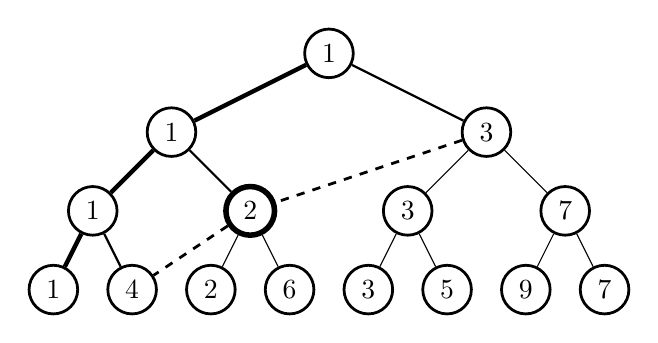
\begin{tikzpicture}[line width = 1pt,
                    solid/.style = {circle, draw, fill = black, minimum size = 0.3cm},
                    empty/.style = {circle, draw, fill = white, minimum size = 0.3cm}]
  \node [empty] (T01) at (6,0) {1};
  \node [empty] (T11) at (4,-1) {1};
  \node [empty] (T12) at (8,-1) {3};
  \node [empty] (T21) at (3,-2) {1};
  \node [empty, line width = 2pt] (T22) at (5,-2) {2};
  \node [empty] (T23) at (7,-2) {3};
  \node [empty] (T24) at (9,-2) {7};
  \node [empty] (T31) at (2.5,-3) {1};
  \node [empty] (T32) at (3.5,-3) {4};
  \node [empty] (T33) at (4.5,-3) {2};
  \node [empty] (T34) at (5.5,-3) {6};
  \node [empty] (T35) at (6.5,-3) {3};
  \node [empty] (T36) at (7.5,-3) {5};
  \node [empty] (T37) at (8.5,-3) {9};
  \node [empty] (T38) at (9.5,-3) {7};
  
  \draw [ultra thick] (T01) -- (T11);
  \draw [thick] (T01) -- (T12);
  \draw [ultra thick] (T11) -- (T21);
  \draw [thick] (T11) -- (T22);
  \draw [thin] (T12) -- (T23);
  \draw [thin] (T12) -- (T24);
  \draw [ultra thick] (T21) -- (T31);
  \draw [thick] (T21) -- (T32);
  \draw [thin] (T22) -- (T33);
  \draw [thin] (T22) -- (T34);
  \draw [thin] (T23) -- (T35);
  \draw [thin] (T23) -- (T36);
  \draw [thin] (T24) -- (T37);
  \draw [thin] (T24) -- (T38);
  
  \draw [dashed] (T12) -- (T22);
  \draw [dashed] (T22) -- (T32);
  \end{tikzpicture} \par
  \end{centering}
  \normalsize

  \section{[TC] Problem 9.3-5}
    Find the median of the array, and use the median as the pivot to partition the array. Determine whether the element you want to find is in the left or right subarray, and calculate its position in the subarray. Recursively doing this, we will find the element we want. \par
    The running time satisfies the recurrence:
    $$T(n) = T(n/2) + \Theta(n)$$ \par
    By the master theorem we get $T(n) = \Theta(n)$.

  \section{[TC] Problem 9.3-7}
  First, calculate the range of the $k$ numbers. For example, the numbers we want can be ranging from the $\lfloor (n-k)/2 \rfloor$-th smallest to the $\lfloor (n-k)/2 \rfloor$ smallest elements. Find the $\lfloor (n-k)/2 \rfloor$-th smallest element in $O(n)$ time, and use it as the pivot to partition the array. Then find the $k$-th smallest element in the right subarray and partition, and the left subarray contains the $k$ elements we want. The total running time is $O(n)$.
  

\end{document}
